% Section owner: Vansh Khod -- test-set validation, discussion and conclusion
\section{Test-Set Validation}\label{sec:test}
The models were retrained on all 100 training engines (10 held out for validation) with three seeds each, and evaluated once on the official test set, with the same protocol as Phase~1. The reported prediction of each network is the average of its three seeds. Phase~1's tuned XGBoost was retrained alongside so that all models are scored on identical rows.

\subsection{Official benchmark}
Table~\ref{tab:test} reports the last-cycle results against the true RUL with 95\% bootstrap intervals over engines. The hybrid scores 11.02 (9.3--12.7), level with XGBoost (10.75, 9.1--12.4), with a slightly lower MAE (8.02 vs.\ 8.09). Its three seeds score 11.05--11.68, so seed variation is of the same size as the differences between the best models. The sequence-only networks score 14.7--15.5: better than XGBoost on raw single-cycle sensors (18.19), but clearly behind the engineered features, the same ranking as in cross-validation.

\begin{table}[t]
\centering
\small
\setlength{\tabcolsep}{4pt}
\caption{Official FD001 test set (last cycle, true RUL)}
\label{tab:test}
\resizebox{\columnwidth}{!}{\begin{tabular}{lccc}
\toprule
Model & RMSE [95\% CI] & MAE & Score \\
\midrule
XGBoost, raw sensors (Ph.~1) & 18.19 [14.9, 21.2] & 12.93 & 963 \\
LSTM, sensor windows & 15.52 [13.0, 18.0] & 11.63 & 463 \\
Transformer, sensor windows & 15.03 [12.7, 17.3] & 11.17 & 367 \\
TCN, sensor windows & 14.72 [12.6, 16.7] & 11.21 & 322 \\
XGBoost, engineered (Ph.~1) & \textbf{10.75 [9.1, 12.4]} & 8.09 & \textbf{161} \\
Hybrid (LSTM + features) & 11.02 [9.3, 12.7] & \textbf{8.02} & 166 \\
\bottomrule
\end{tabular}}
\end{table}

\subsection{Significance}
Because all models are scored on the same engines, we compare them with a paired Wilcoxon signed-rank test~\cite{wilcoxon1945} on per-engine absolute errors, which does not assume normally distributed errors. Each sequence-only network is significantly worse than XGBoost ($p\leq0.0015$; better on only 33--40 of 100 engines). The hybrid and XGBoost are statistically indistinguishable ($p=0.90$; the hybrid is better on 51 engines). Their last-cycle errors are strongly correlated ($r=0.86$): the same engines are hard for both.

\subsection{Error by degradation stage}
Scoring every test cycle (13{,}096 points) against the capped target, the hybrid has a lower RMSE than XGBoost in every stage: early 5.95 vs.\ 6.44, mid 12.33 vs.\ 12.44, late 5.37 vs.\ 5.70, and 8.54 vs.\ 8.81 overall (Fig.~\ref{fig:stage}). Its late-stage bias stays small ($+2.9$ cycles), while the LSTM alone is biased late by $+6.3$ cycles near failure, the dangerous direction. At the last cycle of the 33 engines closest to failure (true RUL $\leq50$), the hybrid has the lowest MAE (2.93, vs.\ 3.38 for XGBoost and 4.39 for the LSTM). Fast-degrading engines remain about 10 cycles late for every model.

\begin{figure}[t]
  \centering
  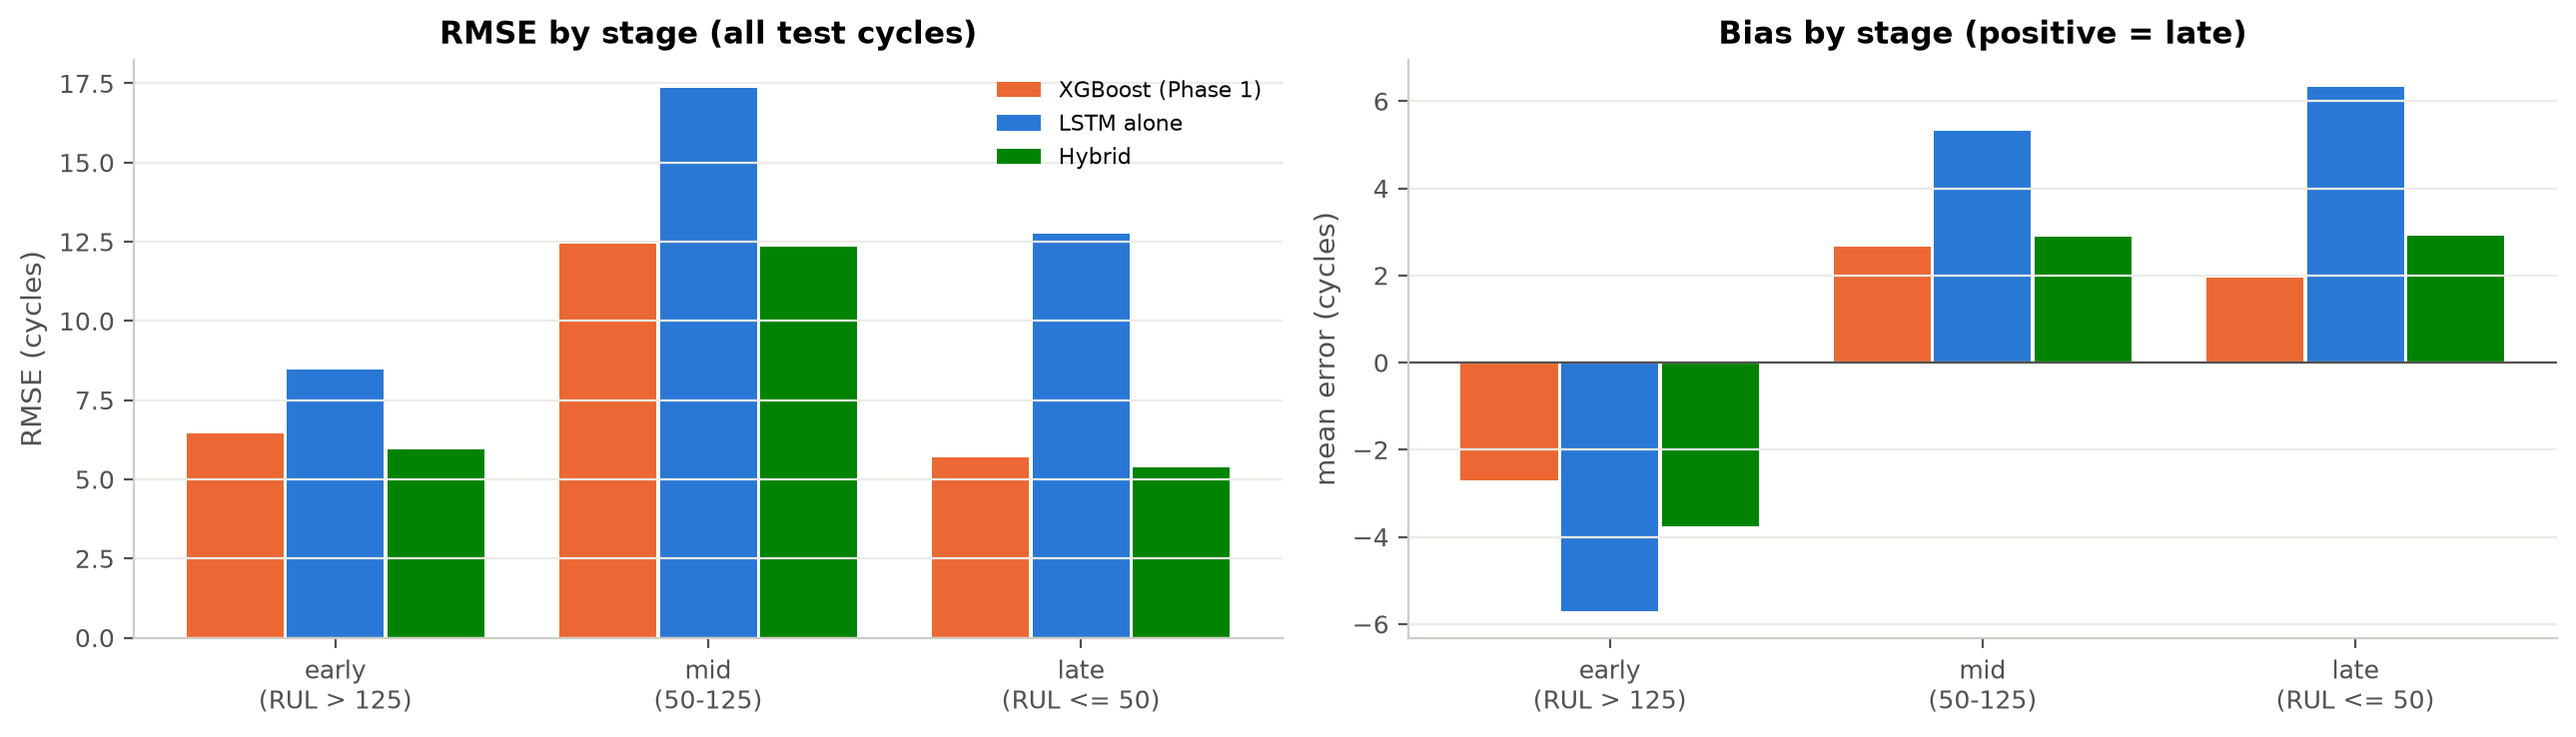
\includegraphics[width=\columnwidth]{10_error_by_stage.png}
  \caption{Test RMSE and bias by degradation stage over all test cycles.}
  \label{fig:stage}
\end{figure}

\subsection{What the sequence branch looks at}
Gradient saliency~\cite{simonyan2014saliency}, the mean $|\partial\hat y/\partial x_{s,\tau}|$ over test windows with RUL $\leq80$ (Fig.~\ref{fig:saliency}), shows that the network concentrates on the last ten or so cycles and on the core speeds $s_9$ (Nc) and $s_{14}$ (NRc), the HPC outlet pressure $s_7$ and the temperature $s_4$. The core speeds were the weakest sensors in Phase~1's ranking and carried little weight in the PCA health index. The sequence branch therefore exploits exactly the signal that the hand-made features use least, which is direct evidence of the complementarity behind the hybrid.

\begin{figure}[t]
  \centering
  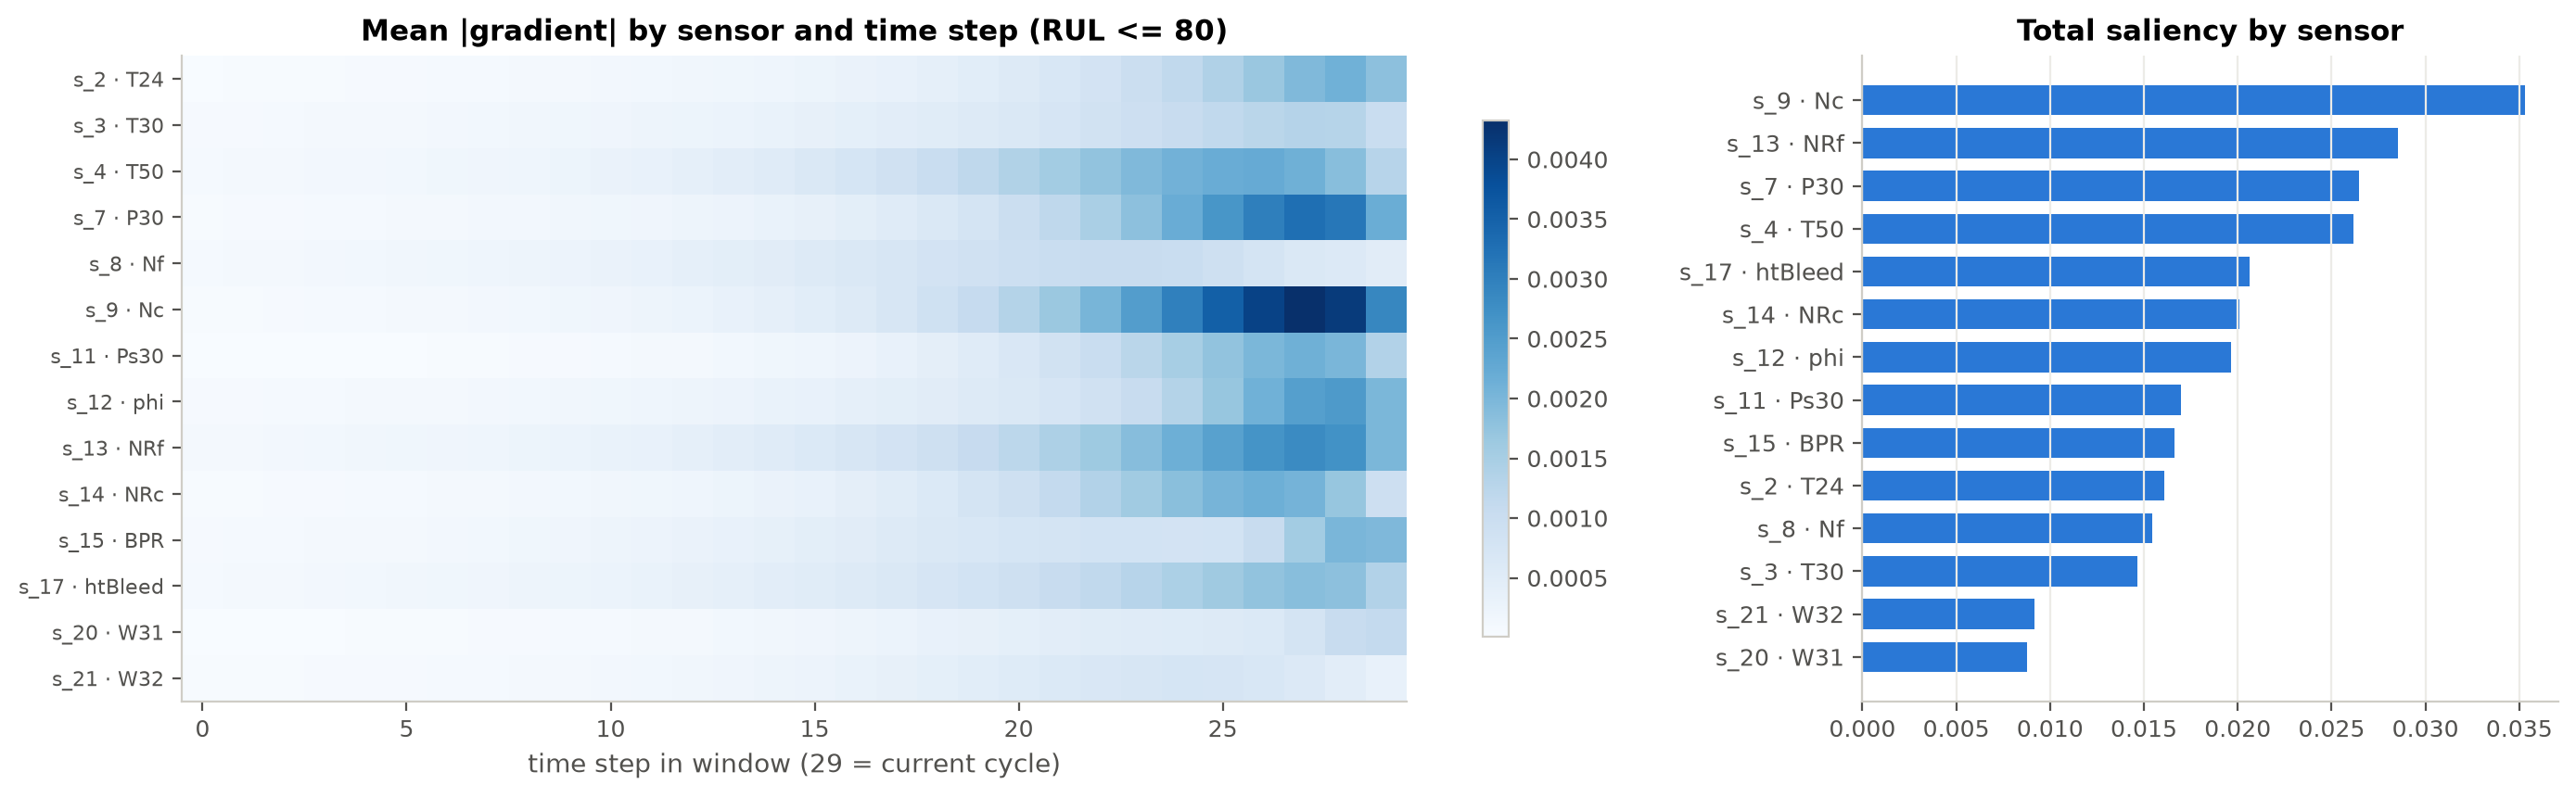
\includegraphics[width=\columnwidth]{10_saliency.png}
  \caption{Gradient saliency of the hybrid's sequence branch by sensor and time step.}
  \label{fig:saliency}
\end{figure}

\section{Discussion and Limitations}
The central comparison of the project has a clear answer on FD001: models that learn only from sensor sequences learn real degradation patterns (3--3.5 cycles better than raw single-cycle features) but do not reach carefully engineered degradation features. The reason is identified by the experiments: the most informative quantities, each engine's distance from its own healthy baseline and its age, lie outside any fixed window, and 100 engines are too few to learn such references. Longer windows help a sequence-only model (14.0 to 11.9 at $W=50$), which supports the brief's hypothesis that fixed windows miss long trajectories. Supplying the context through engineered features helps more.

The hybrid recovers the whole gap, beats both its parts and late fusion in cross-validation, and matches the best feature-based model on the official benchmark, with a small but consistent advantage over all test cycles and near failure. We do not claim a significant improvement over XGBoost: the paired test shows none.

\textbf{Limitations.} FD001 has one operating condition, one fault mode and 100 test engines, so confidence intervals are about $\pm1.7$ cycles wide. Network training is noisy: retraining with another seed moves a CV score by about $\pm0.5$--$0.7$ cycles, as large as most design effects we measured, so only larger effects are claimed. Hyperparameters of the networks were not searched as extensively as XGBoost's in Phase~1, partly for this reason, and early stopping relied on only 7--8 inner-validation engines. Saliency is a local sensitivity measure, not a causal explanation.

\textbf{Future work.} Fast-degrading engines are predicted late by every model, because all of them use the engine's age. Features or targets that express degradation \emph{rate} rather than age, and evaluation on the multi-condition subsets FD002--FD004 (our regime-normalisation pipeline already supports them), are the natural next steps.

\section{Conclusion}
We built a leakage-free sequence-learning pipeline for RUL prediction and compared an LSTM, a temporal CNN and a Transformer encoder with Phase~1's engineered-feature regression under identical engine-level protocols. On their own, the sequence models are significantly worse than the engineered features (test RMSE 14.7--15.5 vs.\ 10.75). A hybrid that fuses an LSTM encoder with the engineered degradation features closes this gap (11.02, statistically level with XGBoost), has the lowest error over all test cycles in every degradation stage, and its sequence branch draws on sensors the features under-use. On 100 engines, domain-informed degradation features remain the backbone of accurate RUL prediction, and sequence learning is most valuable as a complement to them rather than a replacement.
